\documentclass{ximera}

%\usepackage{todonotes}

\newcommand{\todo}{}

\usepackage{esint} % for \oiint
\ifxake%%https://math.meta.stackexchange.com/questions/9973/how-do-you-render-a-closed-surface-double-integral
\renewcommand{\oiint}{{\large\bigcirc}\kern-1.56em\iint}
\fi


\graphicspath{
  {./}
  {ximeraTutorial/}
  {basicPhilosophy/}
  {functionsOfSeveralVariables/}
  {normalVectors/}
  {lagrangeMultipliers/}
  {vectorFields/}
  {greensTheorem/}
  {shapeOfThingsToCome/}
  {dotProducts/}
  {partialDerivativesAndTheGradientVector/}
  {../productAndQuotientRules/exercises/}
  {../normalVectors/exercisesParametricPlots/}
  {../continuityOfFunctionsOfSeveralVariables/exercises/}
  {../partialDerivativesAndTheGradientVector/exercises/}
  {../directionalDerivativeAndChainRule/exercises/}
  {../commonCoordinates/exercisesCylindricalCoordinates/}
  {../commonCoordinates/exercisesSphericalCoordinates/}
  {../greensTheorem/exercisesCurlAndLineIntegrals/}
  {../greensTheorem/exercisesDivergenceAndLineIntegrals/}
  {../shapeOfThingsToCome/exercisesDivergenceTheorem/}
  {../greensTheorem/}
  {../shapeOfThingsToCome/}
  {../separableDifferentialEquations/exercises/}
  {vectorFields/}
}

\newcommand{\mooculus}{\textsf{\textbf{MOOC}\textnormal{\textsf{ULUS}}}}

\usepackage{tkz-euclide}
\usepackage{tikz}
\usepackage{tikz-cd}
\usetikzlibrary{arrows}
\tikzset{>=stealth,commutative diagrams/.cd,
  arrow style=tikz,diagrams={>=stealth}} %% cool arrow head
\tikzset{shorten <>/.style={ shorten >=#1, shorten <=#1 } } %% allows shorter vectors

\usetikzlibrary{backgrounds} %% for boxes around graphs
\usetikzlibrary{shapes,positioning}  %% Clouds and stars
\usetikzlibrary{matrix} %% for matrix
\usepgfplotslibrary{polar} %% for polar plots
\usepgfplotslibrary{fillbetween} %% to shade area between curves in TikZ
%\usetkzobj{all}
\usepackage[makeroom]{cancel} %% for strike outs
%\usepackage{mathtools} %% for pretty underbrace % Breaks Ximera
%\usepackage{multicol}
\usepackage{pgffor} %% required for integral for loops



%% http://tex.stackexchange.com/questions/66490/drawing-a-tikz-arc-specifying-the-center
%% Draws beach ball
\tikzset{pics/carc/.style args={#1:#2:#3}{code={\draw[pic actions] (#1:#3) arc(#1:#2:#3);}}}



\usepackage{array}
\setlength{\extrarowheight}{+.1cm}
\newdimen\digitwidth
\settowidth\digitwidth{9}
\def\divrule#1#2{
\noalign{\moveright#1\digitwidth
\vbox{\hrule width#2\digitwidth}}}




% \newcommand{\RR}{\mathbb R}
% \newcommand{\R}{\mathbb R}
% \newcommand{\N}{\mathbb N}
% \newcommand{\Z}{\mathbb Z}

\newcommand{\sagemath}{\textsf{SageMath}}


%\renewcommand{\d}{\,d\!}
%\renewcommand{\d}{\mathop{}\!d}
%\newcommand{\dd}[2][]{\frac{\d #1}{\d #2}}
%\newcommand{\pp}[2][]{\frac{\partial #1}{\partial #2}}
% \renewcommand{\l}{\ell}
%\newcommand{\ddx}{\frac{d}{\d x}}

% \newcommand{\zeroOverZero}{\ensuremath{\boldsymbol{\tfrac{0}{0}}}}
%\newcommand{\inftyOverInfty}{\ensuremath{\boldsymbol{\tfrac{\infty}{\infty}}}}
%\newcommand{\zeroOverInfty}{\ensuremath{\boldsymbol{\tfrac{0}{\infty}}}}
%\newcommand{\zeroTimesInfty}{\ensuremath{\small\boldsymbol{0\cdot \infty}}}
%\newcommand{\inftyMinusInfty}{\ensuremath{\small\boldsymbol{\infty - \infty}}}
%\newcommand{\oneToInfty}{\ensuremath{\boldsymbol{1^\infty}}}
%\newcommand{\zeroToZero}{\ensuremath{\boldsymbol{0^0}}}
%\newcommand{\inftyToZero}{\ensuremath{\boldsymbol{\infty^0}}}



% \newcommand{\numOverZero}{\ensuremath{\boldsymbol{\tfrac{\#}{0}}}}
% \newcommand{\dfn}{\textbf}
% \newcommand{\unit}{\,\mathrm}
% \newcommand{\unit}{\mathop{}\!\mathrm}
% \newcommand{\eval}[1]{\bigg[ #1 \bigg]}
% \newcommand{\seq}[1]{\left( #1 \right)}
% \renewcommand{\epsilon}{\varepsilon}
% \renewcommand{\phi}{\varphi}


% \renewcommand{\iff}{\Leftrightarrow}

% \DeclareMathOperator{\arccot}{arccot}
% \DeclareMathOperator{\arcsec}{arcsec}
% \DeclareMathOperator{\arccsc}{arccsc}
% \DeclareMathOperator{\si}{Si}
% \DeclareMathOperator{\scal}{scal}
% \DeclareMathOperator{\sign}{sign}


%% \newcommand{\tightoverset}[2]{% for arrow vec
%%   \mathop{#2}\limits^{\vbox to -.5ex{\kern-0.75ex\hbox{$#1$}\vss}}}
% \newcommand{\arrowvec}[1]{{\overset{\rightharpoonup}{#1}}}
% \renewcommand{\vec}[1]{\arrowvec{\mathbf{#1}}}
% \renewcommand{\vec}[1]{{\overset{\boldsymbol{\rightharpoonup}}{\mathbf{#1}}}}

% \newcommand{\point}[1]{\left(#1\right)} %this allows \vector{ to be changed to \vector{ with a quick find and replace
% \newcommand{\pt}[1]{\mathbf{#1}} %this allows \vec{ to be changed to \vec{ with a quick find and replace
% \newcommand{\Lim}[2]{\lim_{\point{#1} \to \point{#2}}} %Bart, I changed this to point since I want to use it.  It runs through both of the exercise and exerciseE files in limits section, which is why it was in each document to start with.

% \DeclareMathOperator{\proj}{\mathbf{proj}}
% \newcommand{\veci}{{\boldsymbol{\hat{\imath}}}}
% \newcommand{\vecj}{{\boldsymbol{\hat{\jmath}}}}
% \newcommand{\veck}{{\boldsymbol{\hat{k}}}}
% \newcommand{\vecl}{\vec{\boldsymbol{\l}}}
% \newcommand{\uvec}[1]{\mathbf{\hat{#1}}}
% \newcommand{\utan}{\mathbf{\hat{t}}}
% \newcommand{\unormal}{\mathbf{\hat{n}}}
% \newcommand{\ubinormal}{\mathbf{\hat{b}}}

% \newcommand{\dotp}{\bullet}
% \newcommand{\cross}{\boldsymbol\times}
% \newcommand{\grad}{\boldsymbol\nabla}
% \newcommand{\divergence}{\grad\dotp}
% \newcommand{\curl}{\grad\cross}
%\DeclareMathOperator{\divergence}{divergence}
%\DeclareMathOperator{\curl}[1]{\grad\cross #1}
% \newcommand{\lto}{\mathop{\longrightarrow\,}\limits}

% \renewcommand{\bar}{\overline}

\colorlet{textColor}{black}
\colorlet{background}{white}
\colorlet{penColor}{blue!50!black} % Color of a curve in a plot
\colorlet{penColor2}{red!50!black}% Color of a curve in a plot
\colorlet{penColor3}{red!50!blue} % Color of a curve in a plot
\colorlet{penColor4}{green!50!black} % Color of a curve in a plot
\colorlet{penColor5}{orange!80!black} % Color of a curve in a plot
\colorlet{penColor6}{yellow!70!black} % Color of a curve in a plot
\colorlet{fill1}{penColor!20} % Color of fill in a plot
\colorlet{fill2}{penColor2!20} % Color of fill in a plot
\colorlet{fillp}{fill1} % Color of positive area
\colorlet{filln}{penColor2!20} % Color of negative area
\colorlet{fill3}{penColor3!20} % Fill
\colorlet{fill4}{penColor4!20} % Fill
\colorlet{fill5}{penColor5!20} % Fill
\colorlet{gridColor}{gray!50} % Color of grid in a plot

\newcommand{\surfaceColor}{violet}
\newcommand{\surfaceColorTwo}{redyellow}
\newcommand{\sliceColor}{greenyellow}




\pgfmathdeclarefunction{gauss}{2}{% gives gaussian
  \pgfmathparse{1/(#2*sqrt(2*pi))*exp(-((x-#1)^2)/(2*#2^2))}%
}


%%%%%%%%%%%%%
%% Vectors
%%%%%%%%%%%%%

%% Simple horiz vectors
\renewcommand{\vector}[1]{\left\langle #1\right\rangle}


%% %% Complex Horiz Vectors with angle brackets
%% \makeatletter
%% \renewcommand{\vector}[2][ , ]{\left\langle%
%%   \def\nextitem{\def\nextitem{#1}}%
%%   \@for \el:=#2\do{\nextitem\el}\right\rangle%
%% }
%% \makeatother

%% %% Vertical Vectors
%% \def\vector#1{\begin{bmatrix}\vecListA#1,,\end{bmatrix}}
%% \def\vecListA#1,{\if,#1,\else #1\cr \expandafter \vecListA \fi}

%%%%%%%%%%%%%
%% End of vectors
%%%%%%%%%%%%%

%\newcommand{\fullwidth}{}
%\newcommand{\normalwidth}{}



%% makes a snazzy t-chart for evaluating functions
%\newenvironment{tchart}{\rowcolors{2}{}{background!90!textColor}\array}{\endarray}

%%This is to help with formatting on future title pages.
\newenvironment{sectionOutcomes}{}{}



%% Flowchart stuff
%\tikzstyle{startstop} = [rectangle, rounded corners, minimum width=3cm, minimum height=1cm,text centered, draw=black]
%\tikzstyle{question} = [rectangle, minimum width=3cm, minimum height=1cm, text centered, draw=black]
%\tikzstyle{decision} = [trapezium, trapezium left angle=70, trapezium right angle=110, minimum width=3cm, minimum height=1cm, text centered, draw=black]
%\tikzstyle{question} = [rectangle, rounded corners, minimum width=3cm, minimum height=1cm,text centered, draw=black]
%\tikzstyle{process} = [rectangle, minimum width=3cm, minimum height=1cm, text centered, draw=black]
%\tikzstyle{decision} = [trapezium, trapezium left angle=70, trapezium right angle=110, minimum width=3cm, minimum height=1cm, text centered, draw=black]


\title{Elementary Functions}

\begin{document}

\begin{abstract}
nice
\end{abstract}
\maketitle












\section*{Elementary Functions}




The Elementary Functions don't do weird things.  They are almost always continuous everywhere (in their domain).  When they do have discontinuities or singularities, they are very nice with obvious jumps.






\begin{itemize} 

\item \textbf{\textcolor{blue!55!black}{Polynomial Function}} 


Polynomials are continuous everywhere. They have no discontinuities or singularities. Constant functions and linear functions are the nicest of the polynomial functions.





\item \textbf{\textcolor{blue!55!black}{Rational Function}} 

Rational functions are continuous everywhere (on their domain).  They have singularities and these are represented with vertical asymptotes and holes on their graphs.  But singularities are not in the domain.  Rational functions are not defined at singularities. Rational functions do not have discontinuities.  They are continuous everywhere (on their domain). 




\item \textbf{\textcolor{blue!55!black}{Radical Function}} 

Radical functions are continuous everywhere.  Not everywhere on the real numbers, because their domains are often not $\mathbb{R}$. Everywhere for functions means everywhere on their domain.






\item \textbf{\textcolor{blue!55!black}{Exponential Function}} 

Basic eE




\item \textbf{\textcolor{blue!55!black}{Shifted Exponential Function}} 

Shifted exponential functions are continuous everywhere (on their domain).




\item \textbf{\textcolor{blue!55!black}{Logarithmic Function}} 

Logarithmic functions are continuous everywhere (on their domain).









\item \textbf{\textcolor{blue!55!black}{Absolute Value Function}} 

The basic absolute value function is continuous everywhere.







\item \textbf{\textcolor{blue!55!black}{Trigonometric Function}} 

Trigonometric functions are continuous everywhere (on their domain).  They have singularities, like tangent, and these singularities are represented with vertical asymptotes on the graphs.  But singularities are not in the domain.  The trigonometric functions are not defined at singularities. Trigonometric functions do not have discontinuities.  They are continuous everywhere (on their domain). 








\end{itemize}




The Elementary Functions are very nice.  They have no discontinuites.  They are continuous everywhere on their domains - or just continuous everywhere - or just continuous.





The first example of a simple function with a discontinuity is the Heaviside step (unit step) function.






\[
Heaviside(x) = 
\begin{cases}
  0 & \text{ on } (-\infty, 0) \\
  \tfrac{1}{2} & \text{ at } 0 \\
  1 & \text{ on } (0, \infty) 
\end{cases}
\]






We also have the \textbf{Greatest Integer} function - also called the \textbf{floor} function.


\[
floor(x) = \lfloor x \rfloor = \, \text{ the greatest integer less than or equal to } \, x
\]





Graph of $y = \lfloor x\rfloor$ is below, except the steps keep going up to the right and down to the left.  The extra 3 dots are a graphical symbol communicating that the pattern continues.
\begin{image}
\begin{tikzpicture}
  \begin{axis}[
            domain=-3:5,
            width=6in,
            height=4in,
            axis lines =middle, xlabel=$x$, ylabel=$y$,
            every axis y label/.style={at=(current axis.above origin),anchor=south},
            every axis x label/.style={at=(current axis.right of origin),anchor=west},
            clip=false,
            %axis on top,
          ]
          \addplot [textColor, very thin, domain=(0:2.3)] {0}; % puts the axis back, axis on top clobbers our open holes
          \addplot [textColor, very thin] plot coordinates {(0,0) (0,2)}; % puts the axis back, axis on top clobbers our open holes
          \addplot [very thick, penColor, domain=(-2:-1)] {-2};
          \addplot [very thick, penColor, domain=(-1:0)] {-1};
          \addplot [very thick, penColor, domain=(0:1)] {0};
          \addplot [very thick, penColor, domain=(1:2)] {1};
          \addplot [very thick, penColor, domain=(2:3)] {2};
          \addplot [very thick, penColor, domain=(3:4)] {3};
          \addplot[color=penColor,fill=penColor,only marks,mark=*] coordinates{(-2,-2)};  %% closed hole          
          \addplot[color=penColor,fill=penColor,only marks,mark=*] coordinates{(-1,-1)};  %% closed hole          
          \addplot[color=penColor,fill=penColor,only marks,mark=*] coordinates{(0,0)};  %% closed hole          
          \addplot[color=penColor,fill=penColor,only marks,mark=*] coordinates{(1,1)};  %% closed hole          
          \addplot[color=penColor,fill=penColor,only marks,mark=*] coordinates{(2,2)};  %% closed hole  
          \addplot[color=penColor,fill=penColor,only marks,mark=*] coordinates{(3,3)};  %% closed hole                  
          \addplot[color=penColor,fill=background,only marks,mark=*] coordinates{(-1,-2)};  %% open hole
          \addplot[color=penColor,fill=background,only marks,mark=*] coordinates{(0,-1)};  %% open hole
          \addplot[color=penColor,fill=background,only marks,mark=*] coordinates{(1,0)};  %% open hole
          \addplot[color=penColor,fill=background,only marks,mark=*] coordinates{(2,1)};  %% open hole
          \addplot[color=penColor,fill=background,only marks,mark=*] coordinates{(3,2)};  %% open hole
          \addplot[color=penColor,fill=background,only marks,mark=*] coordinates{(4,3)};  %% open hole

          \addplot[color=penColor,fill=penColor,only marks,mark=*] coordinates{(3.7,3.5) (3.8,3.6) (3.9,3.7)};  %% 3 dots     
          \addplot[color=penColor,fill=penColor,only marks,mark=*] coordinates{(-1.7,-2.5) (-1.8,-2.6) (-1.9,-2.7)};  %% 3 dots     


        \end{axis}
\end{tikzpicture}
\end{image}












The floor function illustrates a general feeling about elementary functions. The only way discontinities are created is through the use of piecewise defined functions.  To create a discontinuity, we have to break a nice function and just move a piece of it to somewhere else.











\section*{Forcing Discontinuities}



Let's make some discontinuities.

We'll take pieces of different elementary functions and glue them together via piecewise defined functions. 





\begin{example} Jumps







\[
\text{Let } \, G(x) = 
\begin{cases}
  (x+6)(x+2) & \text{ on } (-\infty, -3] \\
  2\sin(x) & \text{ on } (-3, 4) \\
  2 & \text{ at } 4 \\
  2(x-4)-3 & \text{ on } (4, \infty) 
\end{cases}
\]



\begin{image}
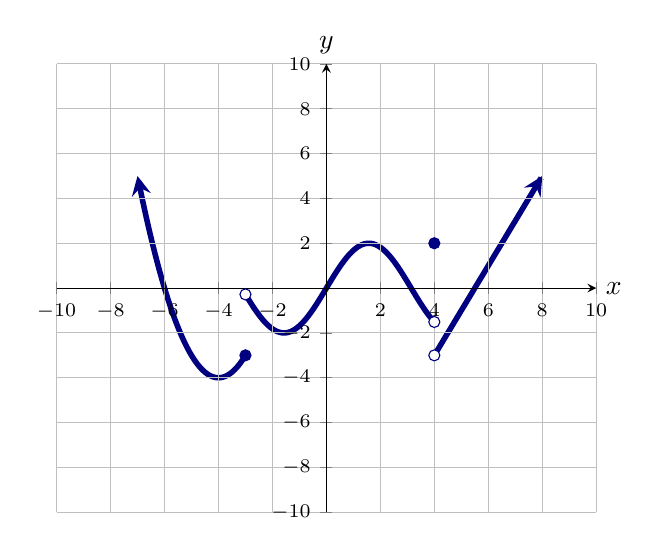
\begin{tikzpicture}
  \begin{axis}[
            domain=-10:10, ymax=10, xmax=10, ymin=-10, xmin=-10,
            axis lines =center, xlabel={$x$}, ylabel={$y$}, grid = major,
            ytick={-10,-8,-6,-4,-2,2,4,6,8,10},
          	xtick={-10,-8,-6,-4,-2,2,4,6,8,10},
          	yticklabels={$-10$,$-8$,$-6$,$-4$,$-2$,$2$,$4$,$6$,$8$,$10$}, 
          	xticklabels={$-10$,$-8$,$-6$,$-4$,$-2$,$2$,$4$,$6$,$8$,$10$},
            ticklabel style={font=\scriptsize},
            every axis y label/.style={at=(current axis.above origin),anchor=south},
            every axis x label/.style={at=(current axis.right of origin),anchor=west},
            axis on top
          ]
          
      		\addplot [line width=2, penColor, smooth,samples=100,domain=(-7:-3),<-] {(x+6)*(x+2)};
          \addplot [line width=2, penColor, smooth,samples=100,domain=(-3:4)] {2*sin(deg(x))};
          \addplot [line width=2, penColor, smooth,samples=100,domain=(4:8),->] {2*(x-4)-3};

      		%\addplot[color=penColor,fill=penColor2,only marks,mark=*] coordinates{(-6,9)};
      		\addplot[color=penColor,fill=penColor,only marks,mark=*] coordinates{(-3,-3)};
          \addplot[color=penColor,fill=penColor,only marks,mark=*] coordinates{(4,2)};

      		\addplot[color=penColor,fill=white,only marks,mark=*] coordinates{(-3,-0.282)};
      		\addplot[color=penColor,fill=white,only marks,mark=*] coordinates{(4,-1.51)};
          \addplot[color=penColor,fill=white,only marks,mark=*] coordinates{(4,-3)};


           

  \end{axis}
\end{tikzpicture}
\end{image}


\begin{itemize}
\item $G$ is continuous on $(-\infty,-3]$, because $G$ is a quadratic function on this interval.
\item $G$ is continuous on $(-3,4]$, because $G$ is a sine function on this interval.
\item $G$ is continuous on $(4,\infty)$, because $G$ is a linear function on this interval.
\end{itemize}


\end{example} 

Basic elementary functions are continuous (on their domains). \\

As we will see when studying compositions in more detail, if you compose a nice basic elementary function with a discontinuous function, then you usually get a discontinuous function.  If you break the domain up into pieces, then the range will follow suit.


























\begin{center}
\textbf{\textcolor{green!50!black}{ooooo-=-=-=-ooOoo-=-=-=-ooooo}} \\

more examples can be found by following this link\\ \link[More Examples of Continuity]{https://ximera.osu.edu/csccmathematics/precalculus1/precalculus1/continuity/examples/exampleList}

\end{center}







\end{document}
